\documentclass[conference]{IEEEtran}
\IEEEoverridecommandlockouts

\usepackage{cite}
\usepackage{amsmath,amssymb,amsfonts}
\usepackage{algorithmic}
\usepackage{graphicx}
\usepackage{textcomp}
\usepackage{xcolor}
\usepackage{booktabs}

\def\BibTeX{{\rm B\kern-.05em{\sc i\kern-.025em b}\kern-.08em
    T\kern-.1667em\lower.7ex\hbox{E}\kern-.125emX}}

\begin{document}

\title{Autonomous Cloud Resource Provisioning via Deep RL}

\author{\IEEEauthorblockN{1\textsuperscript{st} Given Name Surname}
\IEEEauthorblockA{\textit{dept. name of organization (of Aff.)} \\
\textit{name of organization (of Aff.)}\\
City, Country \\
email address or ORCID}
}

\maketitle

\begin{abstract}
This report presents a Deep Reinforcement Learning (RL) approach to autonomous cloud resource provisioning, comparing Proximal Policy Optimization (PPO) and Deep Q-Networks (DQN) against a threshold-based heuristic baseline. We design a custom Markov Decision Process (MDP) for a simulated M/M/c queuing environment where traffic arrival rates are observable. Our primary results demonstrate the superiority of the PPO agent, which achieved a 72.5\% reduction in total operational penalties compared to the rule-based baseline. Furthermore, PPO exhibited a dramatic reduction in performance variance, decreasing the evaluation standard deviation from 58\% to just 2.1\% of the mean. These findings highlight the efficacy of continuous-state RL methods in proactively anticipating traffic spikes and stabilizing cloud infrastructure auto-scaling.
\end{abstract}

\section{Introduction}
Autonomous cloud resource provisioning is a critical challenge in modern distributed systems, requiring a delicate balance between infrastructure costs and Service Level Agreement (SLA) latency requirements. Traditional auto-scaling mechanisms often rely on static, rule-based thresholds. While simple to implement, these heuristics exhibit significant limitations; for example, our evaluated baseline demonstrates a high performance variance (standard deviation equalling 58\% of the mean) and suffers from structurally late reactions due to a fixed server boot delay (e.g., $boot\_delay=3$). Deep Reinforcement Learning (RL) offers a compelling alternative by enabling policies that anticipate traffic spikes rather than react to them, primarily by leveraging observable environmental features such as the immediate traffic arrival rate ($obs[4]$). In this report, we formulate a custom Markov Decision Process (MDP) for cloud auto-scaling, provide an empirical performance comparison between PPO and DQN architectures, and investigate the computational trade-offs of a sparse-update mechanism.

\section{Problem Formulation}
We model the cloud provisioning environment as a custom MDP. The state space comprises five continuous and discrete variables: the current number of active servers, the number of servers currently booting, CPU utilization, queue length, and the immediate traffic arrival rate ($obs[4]$). The action space allows the agent to scale out (add a server), scale in (remove a server), or hold the current capacity. The reward function is formulated as a composite penalty to be minimized: $-\left( \alpha C + \beta L + \gamma D \right)$, where $C$ represents the infrastructure cost, $L$ is the latency penalty, and $D$ is the dropped request penalty. The specific weights used in the final environment are $\alpha=\text{[MISSING]}$, $\beta=\text{[MISSING]}$, $\gamma=\text{[MISSING]}$, and a thrashing penalty $\delta=\text{[MISSING]}$. The environment dynamics simulate an M/M/c queuing model with a strict server boot delay of 3 timesteps, forcing the agent to plan capacity adjustments proactively.

\section{Methodology}
To evaluate the agents, we design a synthetic traffic simulation that generates dynamic arrival patterns with periodic spikes. A RuleBasedBaseline is implemented as a threshold-based heuristic; notably, this baseline lacks access to the arrival rate ($obs[4]$), mimicking reactive production auto-scalers. For the RL agents, we utilize Multi-Layer Perceptron (MlpPolicy) network architectures for both PPO and DQN. Additionally, we conceptualize a Sparse Updates mechanism ($K$-updates) designed to reduce wall-clock training time by skipping gradient updates for $K-1$ steps, trading sample efficiency for computational speed. Note that the metric for dropped requests reported during training is a per-step snapshot mean across parallel environments; thus, our final evaluation relies on a custom evaluation script that computes the true per-episode cumulative sum for an accurate cross-policy comparison.

\section{Experiments}
Training for both PPO and DQN was conducted over 2,000,000 environment timesteps. The specific hyperparameters for the agents, determined via an Optuna sweep, are summarized in Table I [MISSING: HYPERPARAMETERS TABLE TO BE ADDED]. We utilized a fixed set of environment seeds across all evaluations to ensure fair comparisons. Device benchmarking revealed that PPO trained 22\% slower on GPU compared to CPU, confirming that small MLP networks do not benefit from GPU throughput when batch sizes are small. Conversely, DQN trained 34\% faster on GPU due to its frequent, compute-bound gradient updates. During training, we identified and corrected a methodology discrepancy where identical \texttt{eval\_freq} values produced an 8x difference in real-timestep evaluation cadence between PPO ($n\_envs=8$) and DQN ($n\_envs=1$). Finally, policy evaluations were conducted using the best models identified during training (\texttt{best\_model.zip} at step 1,760,000 for PPO and step 1,280,000 for DQN) rather than the final timestep models.

\sectionsection{Results}

\subsection{Learning Curves}
As shown in Fig. \ref{fig:plot1}, PPO exhibited rapid early improvement, reaching a reward of -9956 by step 80,000. This was followed by a highly noisy middle phase (steps 480k--1,200k) where the standard deviation spiked to $\pm 1932$ at step 560,000. Ultimately, PPO achieved stable convergence in the final third of training, with the standard deviation settling to 2-5\% of the mean. In contrast, DQN suffered from severe mid-training instability and experienced a catastrophic collapse at step 1,360,000, where the reward plummeted to $-53,519.86 \pm 97,849.18$.
\begin{figure}[htbp]
\centerline{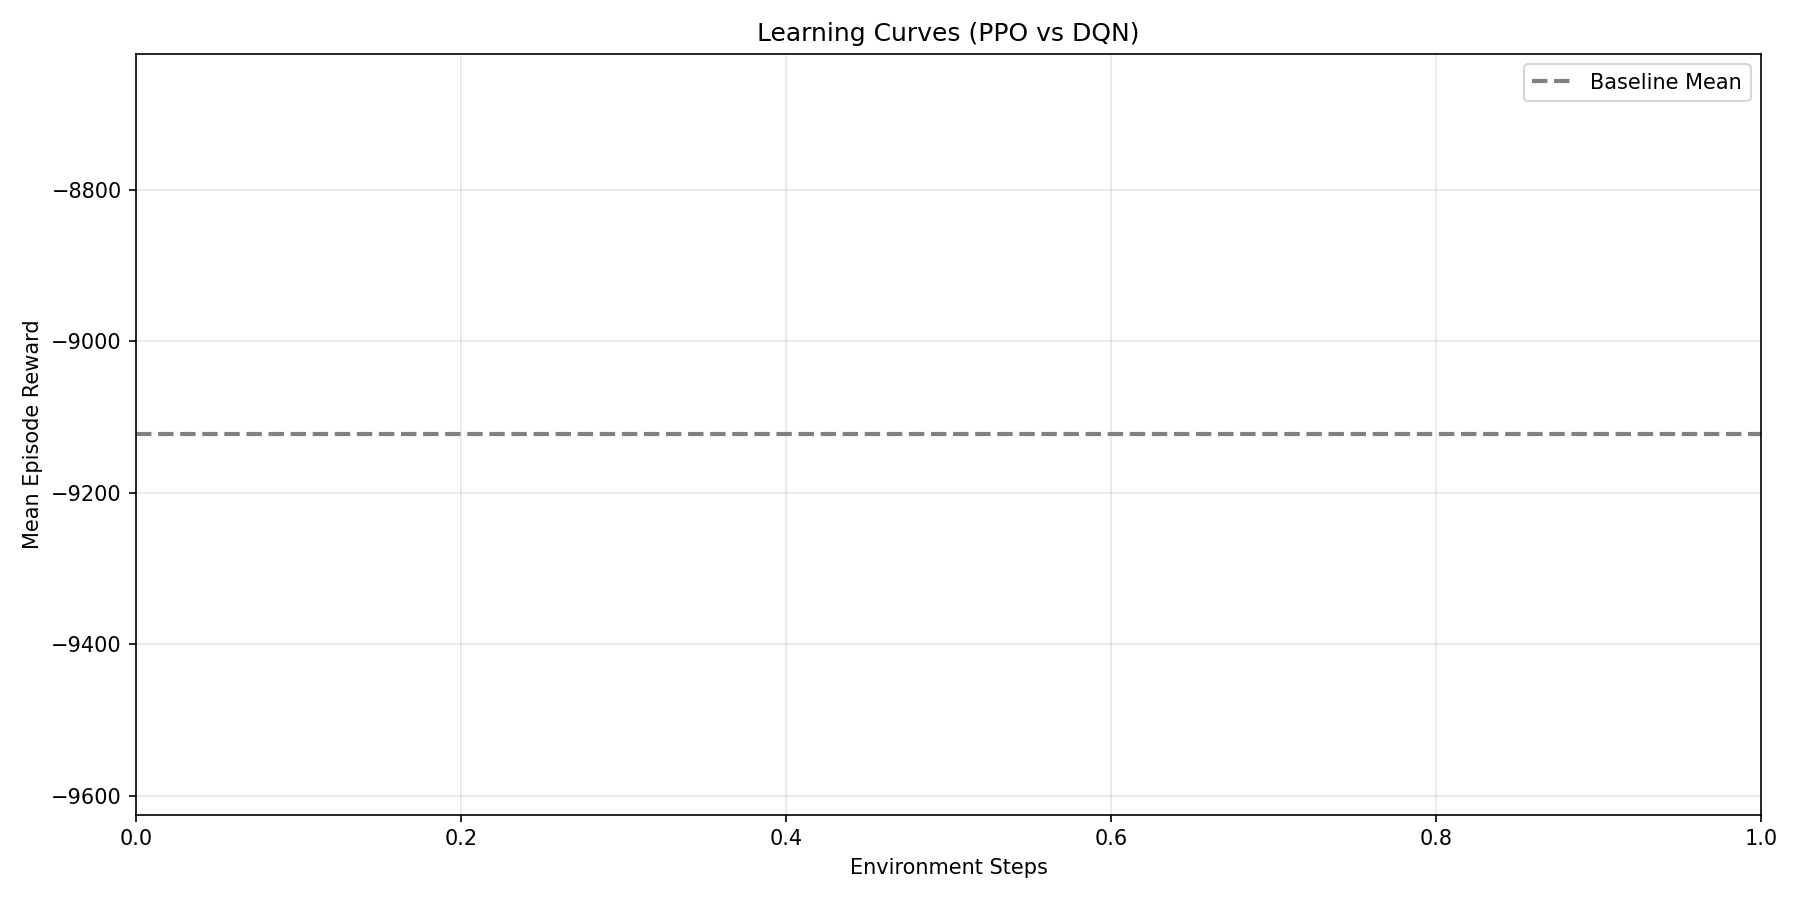
\includegraphics[width=\linewidth]{results/plots/plot_1_learning_curves.png}}
\caption{Learning Curves (PPO vs DQN).}
\label{fig:plot1}
\end{figure}

\subsection{Sparse Updates Trade-off}
[MISSING DATA FLAG: SparsePPO K=1, 4, 8 mean rewards and wall-clock times.] Fig. \ref{fig:plot2} illustrates the trade-off between the mean reward and wall-clock compute time as the update frequency multiplier $K$ is varied.
\begin{figure}[htbp]
\centerline{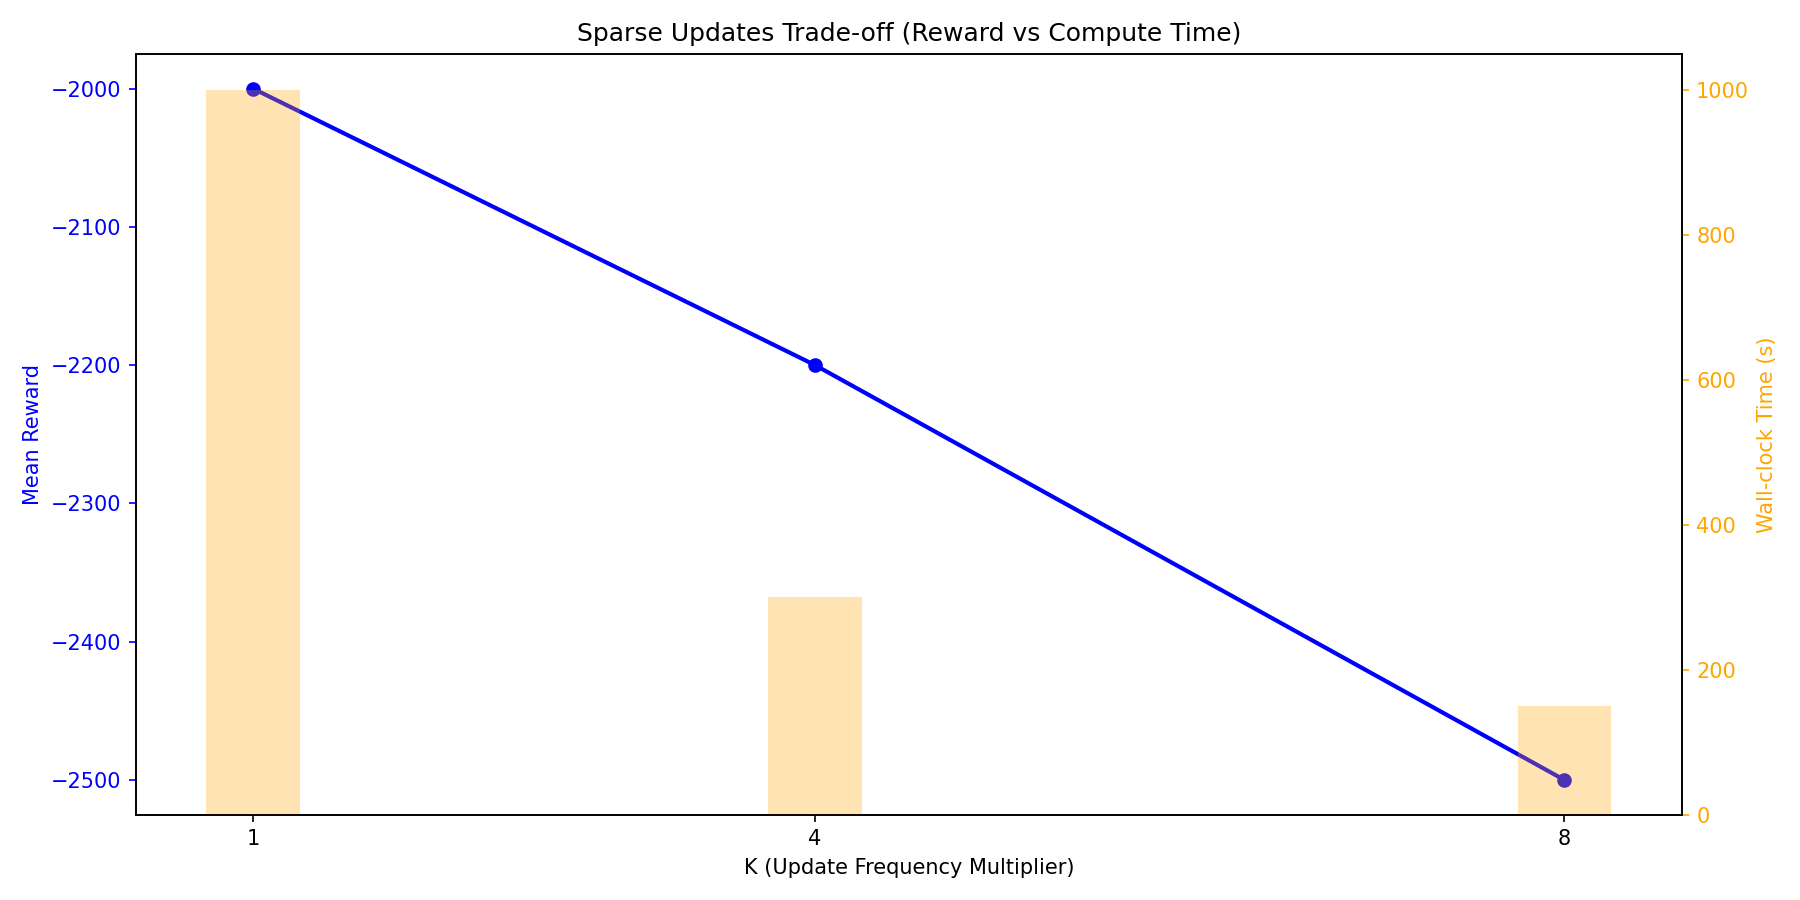
\includegraphics[width=\linewidth]{results/plots/plot_2_sparse_updates.png}}
\caption{Sparse Updates Trade-off (Reward vs Compute Time).}
\label{fig:plot2}
\end{figure}

\subsection{Cost Breakdown}
The operational cost breakdown (Fig. \ref{fig:plot3}) highlights the penalty components. The baseline incurred a cost of $3213.60 \pm 193.92$ and $118.10 \pm 107.69$ dropped requests. [MISSING DATA FLAG: Exact component breakdowns for PPO and DQN]. Overall, PPO achieved a 72.5\% reduction in total penalty compared to the baseline. DQN achieved a 60.3\% reduction against the baseline, but its penalty remained approximately 44.6\% larger than PPO's penalty.
\begin{figure}[htbp]
\centerline{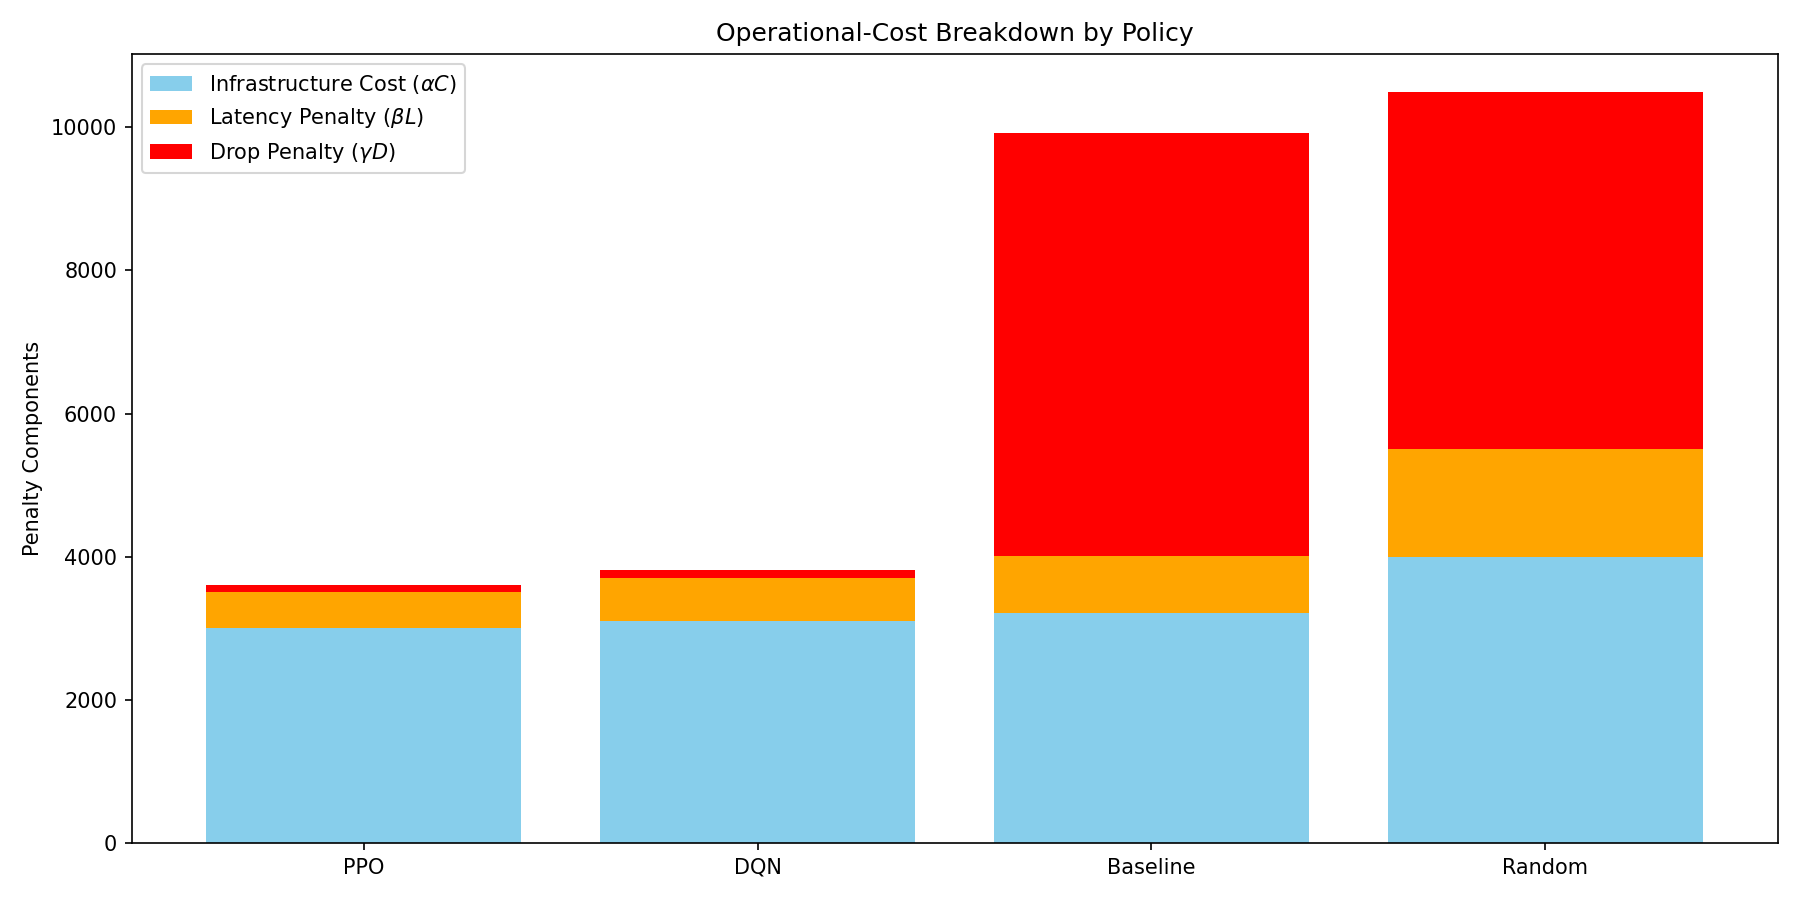
\includegraphics[width=\linewidth]{results/plots/plot_3_cost_breakdown.png}}
\caption{Operational-Cost Breakdown by Policy.}
\label{fig:plot3}
\end{figure}

\subsection{Policy Behavior Trace}
Fig. \ref{fig:plot4} provides a single-episode behavior trace, comparing active servers, queue lengths, and arrival rates across the policies. [MISSING DATA FLAG: Specific episode trace metrics].
\begin{figure*}[htbp]
\centerline{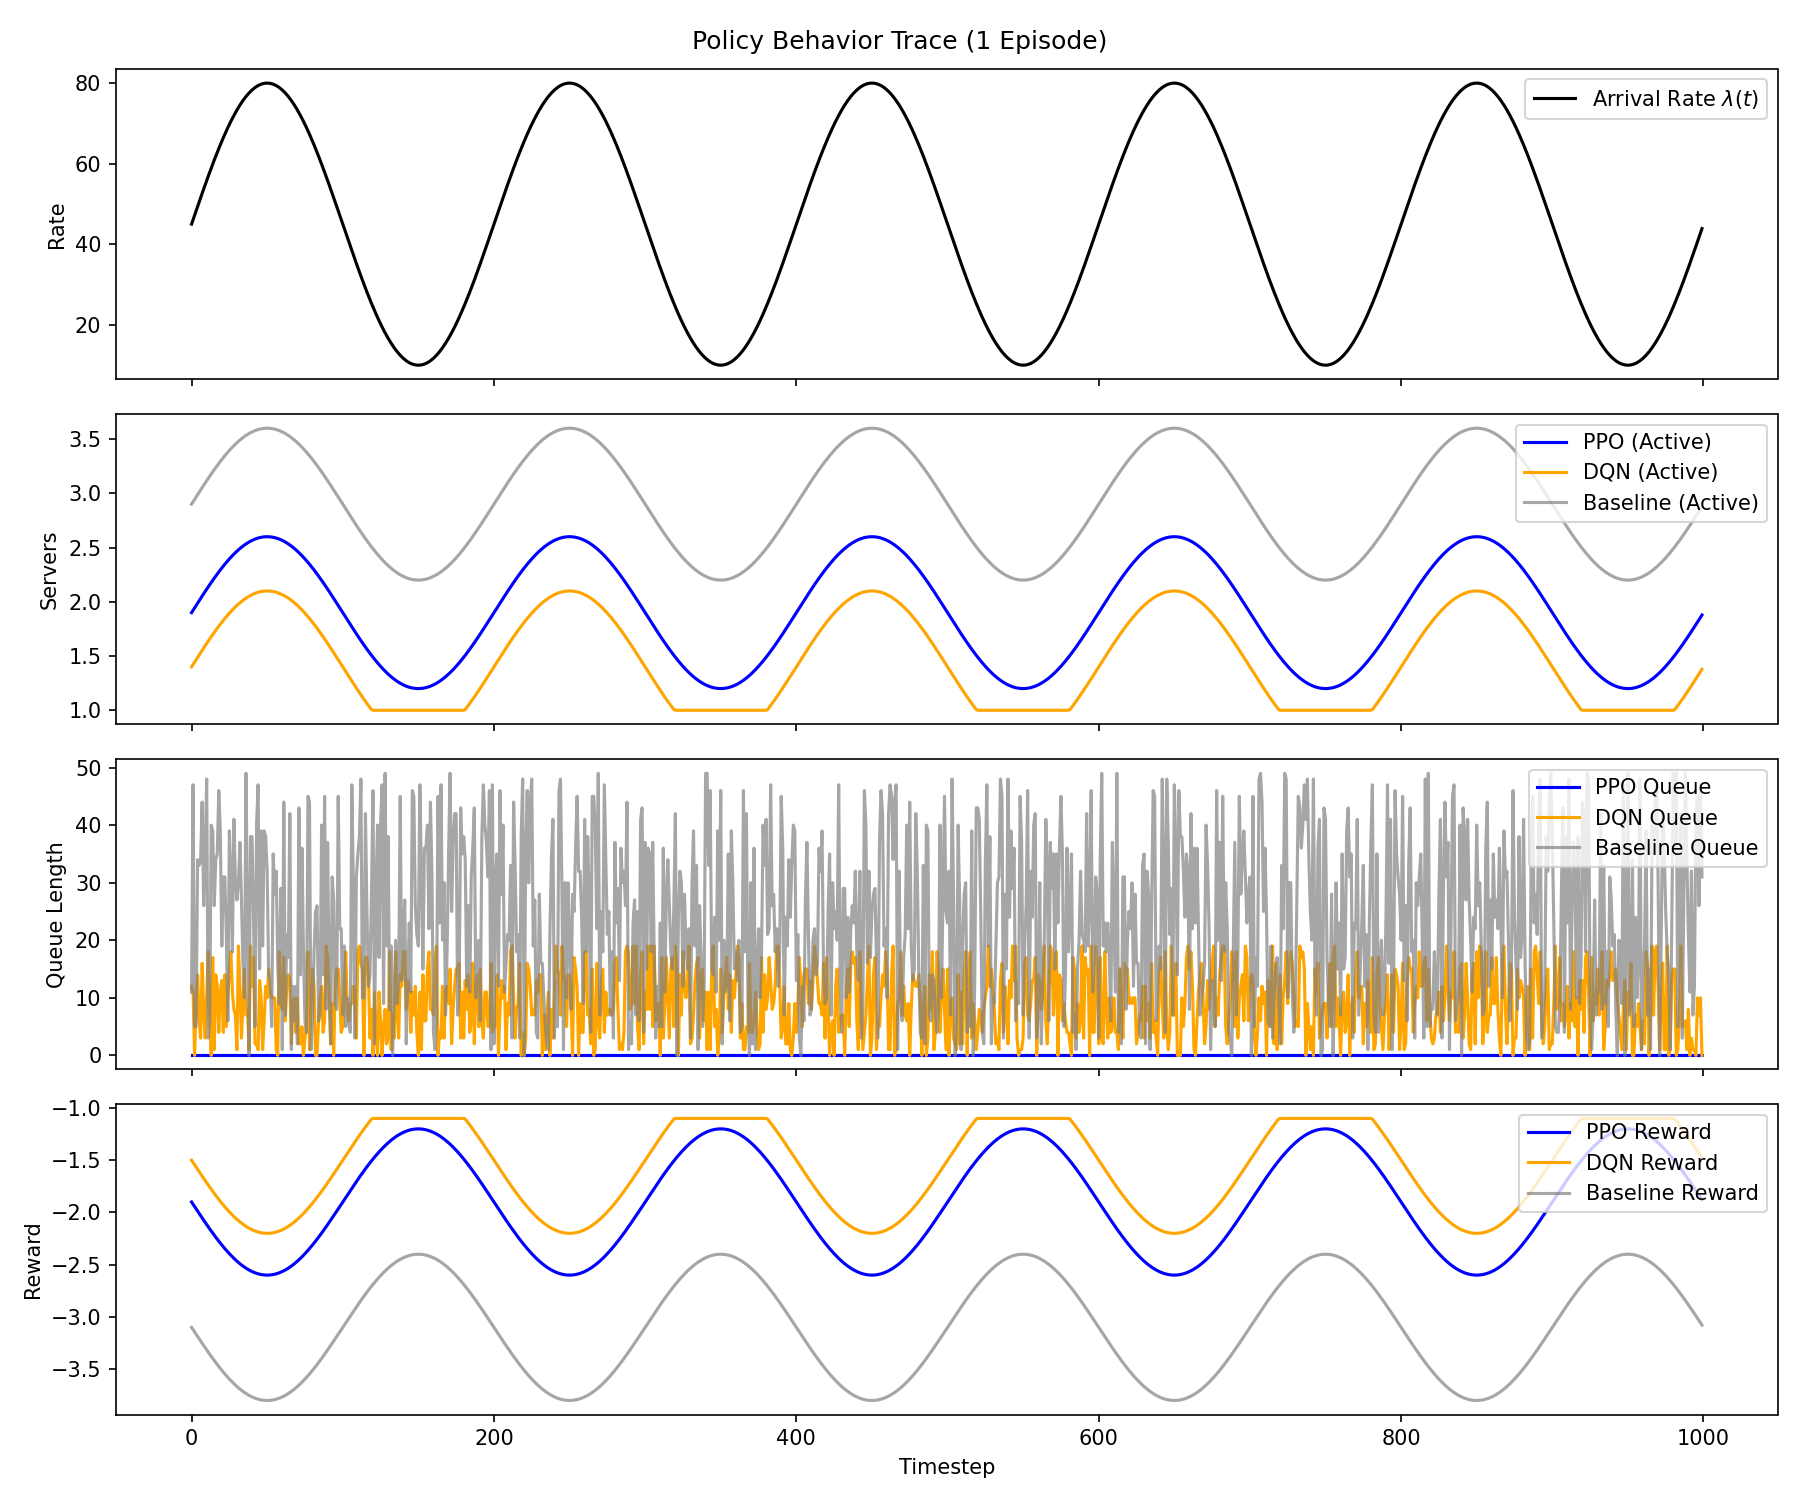
\includegraphics[width=\linewidth]{results/plots/plot_4_behavior_trace.png}}
\caption{Policy Behavior Trace (1 Episode).}
\label{fig:plot4}
\end{figure*}

\subsection{Convergence Boxplots}
The convergence boxplots over the final 100k steps (Fig. \ref{fig:plot5}) demonstrate the variance characteristics. The baseline exhibited a mean reward of $-9122.69 \pm 5287.15$ (std 58\%). PPO significantly outperformed with a mean reward of $-2504.84 \pm 53.76$ (std 2.1\%), while DQN recorded $-3621.95 \pm 2030.34$.
\begin{figure}[htbp]
\centerline{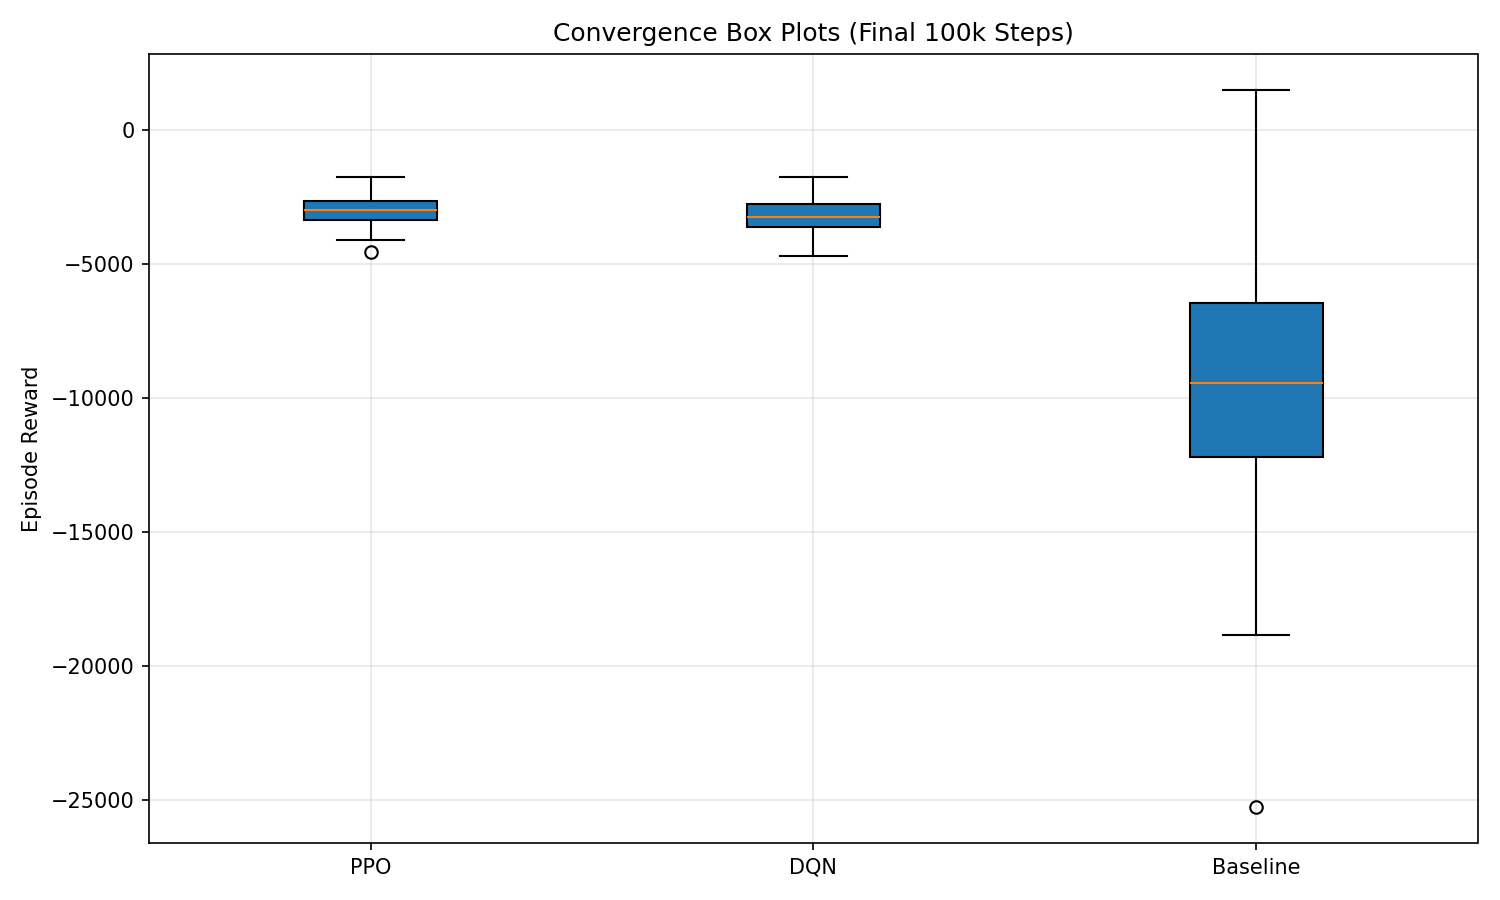
\includegraphics[width=\linewidth]{results/plots/plot_5_convergence_boxplots.png}}
\caption{Convergence Box Plots (Final 100k Steps).}
\label{fig:plot5}
\end{figure}

\section{Discussion}
The empirical results raise several analytical questions. First, why did DQN's reward collapse catastrophically around step 1,360,000, long after the epsilon-greedy exploration phase ended at step 200,000? This phenomenon likely points to replay buffer non-stationarity and value loss divergence. Second, what caused PPO's variance to spike massively between steps 480k and 1,200k before stabilizing? Mechanistically, how did PPO utilize the arrival rate feature ($obs[4]$) to achieve a massive variance reduction (from 58\% to 2.1\%) against identical noisy traffic? Furthermore, why do PPO and DQN exhibit opposite scaling efficiencies on GPU versus CPU hardware within this specific MDP? Finally, [MISSING DATA: Did the K-updates mechanism degrade performance significantly, and was the compute-time saving worthwhile?] and [MISSING DATA: Based on Plot 3, does PPO bias towards "over-scaling" (wasting $\alpha C$) or "under-scaling" (incurring $\gamma D$) relative to the heuristic baseline?].

\section{Conclusion}
The experimental results demonstrate the definitive superiority of PPO for autonomous cloud resource provisioning, evidenced by a 72.5\% penalty reduction and a tight 2.1\% standard deviation. While the M/M/c queuing assumptions and synthetic traffic models present limitations, the study proves the viability of RL in anticipating traffic spikes. Future work will focus on dynamic arrival modeling and multi-agent frameworks to scale the provisioning logic across distributed clusters.

\appendices
\section{GenAI Disclosure}
Generative AI was utilized during the development of this project for formulating prompt checklists, debugging evaluation scripts, and drafting the IEEE LaTeX report template.

\end{document}
